
\section{Protein as Second Language}

We introduce ``Protein-as-Second-Language'', a framework that treats amino-acid sequences as a new symbolic system to be learned much like humans acquire a foreign language. Just as learners infer the meaning of unfamiliar words by repeatedly encountering them in context, we construct a \textbf{\textit{protein–natural language bilingual dataset}} (Sec.~\ref{sec:dataset}) and design an \textbf{\textit{adaptive context construction mechanism}} (Sec.~\ref{sec:framwork}) to provide such contextual exposure. In this way, our framework enables LLMs to acquire protein semantics through exemplars rather than through extensive re-training.

\subsection{Bilingual Dataset Construction}
\label{sec:dataset}

We curate our bilingual dataset in three steps (Figure~\ref{fig:pipline}). Starting from 573,661 Swiss-Prot~\cite{bairoch2000swiss} entries with gene ontology (GO) annotations, we avoid directly converting all annotations, as this would introduce heavy redundancy; instead, we construct a balanced sample. Specifically, (i) we prune the GO-directed acyclic graph (GO-DAG) to obtain representative functional categories and group proteins accordingly (Sec.~\ref{sec:step1}), (ii) perform bilingual deduplication by clustering sequences within each protein group and sampling proteins with diverse functional annotation (Sec.~\ref{sec:step2}), and (iii) use DeepSeek-R1~\cite{guo2025deepseek} to generate attribute, knowledge, descriptive, and true/false QA pairs, yielding 79,926 high-quality protein–QA triples (Sec.~\ref{sec:step3}).

\begin{figure}[ht]
\centering
\includegraphics[width=\linewidth]{figure/data_construction_0.pdf}
\caption{\textbf{The overview of data construction of our bilingual protein–QA dataset.}}
\label{fig:pipline}
\end{figure}

\subsubsection{Function-Based Grouping}
\label{sec:step1}

To enable representative sampling across functional categories, the dataset is partitioned according to the GO hierarchy. Directly using the raw directed acyclic graph (DAG) risks over-fragmentation from overly fine, sparsely populated terms, and excessive generalization near the root. To address this, we adapt a pruning strategy inspired by decision tree simplification~\cite{mondon1984classification}, where complexity is managed through a penalty to avoid overfitting. This strategy aims to retain an optimal set of GO terms as functional grouping nodes. It balances granularity and coverage, ensuring that the retained nodes represent biologically diverse yet statistically well-supported categories for downstream sampling.

The pruning process is driven by two main criteria:
% \begin{itemize}
% \item 
(1) A node is retained if it meets the \textit{\textbf{minimum support threshold}}, which ensures that the node has a sufficient number of associated proteins, and does not exhibit significant child imbalance.
% \item 
(2) If the \textit{\textbf{child-imbalance ratio}} is high, meaning the protein distribution among a node's child terms is uneven, the parent node is retained, even if the child nodes fail to meet the minimum support threshold.
% \end{itemize}

\paragraph{Minimum Support Threshold}
A node is retained only if the number of associated proteins meets a depth-adjusted threshold $m(d)$, which adapts based on the node's depth in the GO hierarchy. The threshold is calculated as:
\begin{equation}
m(d) = \lambda \cdot C_{tot}\cdot(1+\beta d)
\end{equation}
where $C_{tot}$ is the total protein count, $d$ is the node depth, and $\lambda$ and $\beta$ are constants. This dynamic threshold is designed to prevents deep nodes from splitting infinitely due to overly small absolute values.

\paragraph{Child-Imbalance Ratio}
The child-imbalance ratio is applied to assess whether the child nodes of a given term are too imbalanced. The imbalance ratio $\rho(v)$ is computed as the ratio of the largest to the smallest protein count among the child nodes: 

\begin{equation}
p(u)=\frac{\displaystyle\max_{u\in C^{+}(v)} C(u)}
          {\displaystyle\min_{u\in C^{+}(v)} C(u)}
\end{equation}

where $C^{+}(v)$ represents the set of valid child nodes with non-zero protein counts. If the imbalance ratio $\rho(v)$ exceeds a specified threshold $\tau(d)$, the parent node $v$ is retained to preserve the biological diversity. This threshold is adjusted dynamically with the depth $d$ to allow for greater flexibility at deeper levels of the hierarchy:

\begin{equation}
\tau(d) = \tau_0 \cdot \alpha^d
\end{equation}
where $\tau_0$ is the base threshold, and $\alpha$ is a scaling factor.

By applying these two criteria, the pruning process is carried out recursively, allowing the algorithm to adaptively prune the GO DAG and identify the most relevant, biologically diverse functional groups.

\subsubsection{Bilingual deduplication }
\label{sec:step2}

After grouping by GO term, proteins within the same node often exhibit high similarity, as they represent homologous proteins. 
% 
To address this, we use MMseqs2~\cite{steinegger2017mmseqs2} for sequence clustering within each GO node, applying a 70\% \textbf{\textit{amino acid sequence similarity}} threshold. From each cluster, a single representative sequence is selected. This threshold efficiently removes redundant sequences with minimal functional variation while preserving functional diversity.

While sequence similarity-based redundancy removal effectively reduces sequence-level redundancy, it does not necessarily capture functional divergence. Specifically, sequence similarity below 70\% does not imply functional divergence, and substantial functional redundancy may still exist within the set~\cite{devos2000practical}. To address this, we focus on \textbf{\textit{annotation semantic similarity}}, quantifying the functional relationships between proteins based on their GO annotations. Inspired by the simGIC method~\cite{pesquita2008metrics} for calculating GO terms semantic similarity, we calculate the Protein Functional Information Content $\mathrm{IC}_{\text{protein function}}$ for each protein, which is the sum of the Information Content (IC) of all associated GO terms and their ancestral terms. The IC of each GO term is calculated based on its frequency in the dataset, using the total protein set after sequence redundancy removal. The $\mathrm{IC}_{\text{protein function}}$ value for each Protein ID is computed as:

\begin{equation}
\text{IC}_{\text{protein function}} = \sum_{g \in \text{GO terms of } p} \text{IC}(g) + \sum_{g' \in \text{ancestors of GO terms of } p} \text{IC}(g').
\end{equation}

This provides a quantitative measure of each protein's functional information, capturing both direct and indirect annotations. For each GO term, proteins are sampled based on their unique $\mathrm{IC}_{\text{protein function}}$ values (rounded to 3 decimal places). To ensure balanced species representation, a species quota strategy is applied based on the proportions of Eukaryota, Bacteria, Archaea, and Viruses in the dataset after sequence redundancy removal. This ensures an unbiased species distribution in the final sample.
% 
The bilingual deduplication process reduces redundancy in two aspects, amino acid sequence and annotation semantics, ensuring a balanced and diverse protein corpus.

\subsubsection{LLM-based QA Construction}
\label{sec:step3}

To transform curated protein annotations into natural-language question–answer pairs, we prompt the DeepSeek-R1~\cite{guo2025deepseek} model to generate biologically grounded QA texts that reflect both functional attributes and contextual knowledge (the prompts used for each QA type are provided in Appendix~\ref{appendix:llm_prompt}). The resulting QA corpus covers four complementary types:
% 
\blackcircle{1} \textit{Attribute-based QA} captures factual properties directly associated with a protein, such as molecular function, cellular component, or family.
\blackcircle{2} \textit{Knowledge-based QA}  comprises concise, annotation-driven questions and answers that involve in multiple biological aspects of a protein, such as expression, localization, mechanism, and interactions.
\blackcircle{3} \textit{Descriptive Text QA} produces longer natural-language explanations that integrate multiple annotations into coherent functional summaries.
\blackcircle{4} \textit{True or False QA} consists of single statements that integrate multiple biological aspects of a protein, accompanied by a True/False answer and a brief explanation.

These four types yield a rich and varied bilingual dataset, ensuring that models are exposed to both concise factual knowledge and more detailed contextual explanations, supporting their ability to understand and reason about protein functions.

\subsection{Bilingual Contextual Learning}
\label{sec:framwork}
\begin{figure}[ht]
\centering
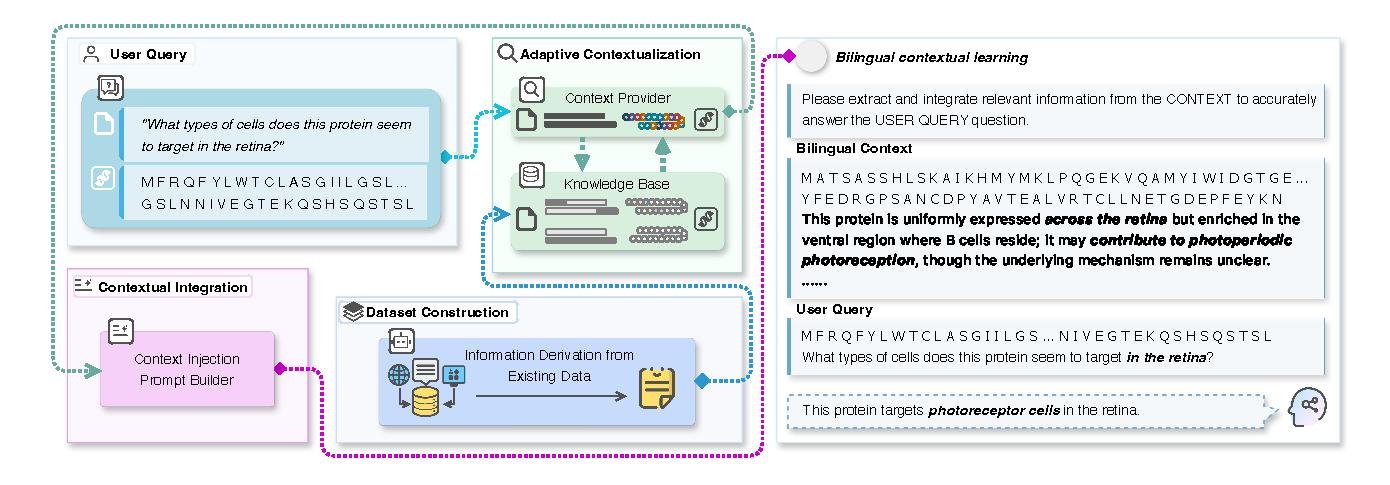
\includegraphics[width=1\linewidth]{figure/context_0.pdf}
\caption{\textbf{Process of Query-Adaptive Context Construction. }}
\label{fig:context}
\end{figure}

In practical scenarios, questions concerning protein sequences are often highly flexible and complex: they require not only analogous proteins with similar sequence patterns to capture potential structural or functional signals, but also complementary descriptive knowledge and QA pairs to provide semantic grounding.
% 
As shown in Figure~\ref{fig:context}, we propose an adaptive context construction mechanism, for \textbf{\textit{bilingual contextual learning}}, designed to selectively build bilingual learning contexts for each query. 
% 
Instead of brute-force mixing of amino acid sequences and descriptive texts, the mechanism follows the principle of second language acquisition—exposing learners to new words in context so that meaning and usage can be inferred~\cite{huckin1999incidental}.
% 
By analogy, LLMs acquire protein semantics and reasoning ability through context-driven exposure that grounds sequence patterns in functional and structural exemplars.

The mechanism operates in three stages. First, the adaptive context provider selects candidate contexts from the protein–natural language bilingual dataset, guided by two criteria: 
(i) amino acid sequence homology between candidate proteins and the query sequence, computed with MMseqs2~\cite{steinegger2017mmseqs2}, and (ii) similarity between the descriptive texts or QA pairs of candidate proteins and the query question.
% 
Second, the contextual integration module structures the selected examples into a coherent context. Finally, the constructed bilingual context is combined with the query and presented to the LLM as in-context examples, enabling analogy-based reasoning and evidence integration to produce biologically meaningful responses.